\documentclass[12pt]{article}
\usepackage[utf8]{inputenc}
\usepackage{amssymb}
\usepackage{amsmath}
\usepackage{graphicx}
\graphicspath{{figs/}}
\title{AI1110 assignment1}
\author{Bhargava Ram Rajulapati, CS21BTECH11052}

\begin{document}
  \maketitle
  \section*{Question 6}
  \begin{figure}[h]
  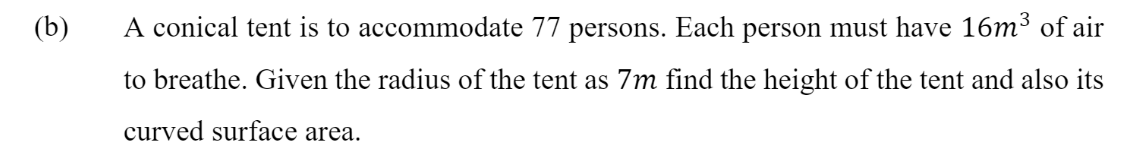
\includegraphics[width=\textwidth]{question.png}
  \end{figure}
  \section*{Solution:}
  Given a conical tent which can accommodate 77 persons and each         
   person must have $16m^3$ of air to breathe.\\
  so the volume of conical tent is,
  \begin{align*}
    v = 77 \times 16 m^3 
  \end{align*}
  we know that volume of conical tent is same as a cone having
  radius $r$,height $h$,
  \begin{align*}
     v = \frac{\pi r^2 h}{3} 
  \end{align*}
  from the question we are given radius of cone, \\
  $ r = 7 m $\\ 
  height of cone is
  \begin{align*}
   h = \frac{3 v}{\pi r^2} 
  \end{align*}
  By substituting values we can get, \\
  $ h = 24 m $ \\\\
  Now we know radius and height so we can find lateral height $l$
  which is given by,
  \begin{align*}
    \hspace*{12pt} l = \sqrt{r^2 + h^2} \\
    \Rightarrow l = \sqrt{7^2 + 24^2} \\
    \Rightarrow l = 25 m
  \end{align*}
  we know that lateral/curved surface area $s$ of a cone is given
  by,
  \begin{align*}
    \hspace*{12pt} s = \pi \times r \times l \\
    \Rightarrow  s = \frac{22}{7} \times 7 \times 25  \\
    \Rightarrow  s = 550 m^2 
  \end{align*}
   
  Hence the curved surface area is $ 550 m^2 $. \\\\
  The output of the program used to find and verify these numbers
  is: \\
  \begin{figure}[h]
  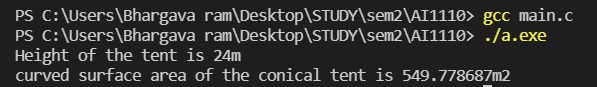
\includegraphics[width=\textwidth]{output.png}
  \caption{output of c code}
  \end{figure}   
\end{document}
